\documentclass[UTF8,zihao=-4,openany]{ctexrep}
\usepackage[a4paper,top=2.5cm,bottom=2.3cm,left=2.8cm,right=2.2cm]{geometry}
\usepackage{amsmath,amssymb}
\usepackage{booktabs,longtable,tabularx,array,multirow}
\usepackage{graphicx,float}
\usepackage{enumitem}
\usepackage{xcolor}
\usepackage{tikz}
\usetikzlibrary{arrows.meta,positioning,shapes.geometric,calc}
\usepackage{fancyhdr,lastpage}
\usepackage{hyperref}
\usepackage{caption}
\usepackage{setspace}
\usepackage{pdfpages}

\setCJKmainfont{Songti SC}
\setCJKsansfont{Heiti SC}
\setCJKmonofont{Kaiti SC}
\setmainfont{Times New Roman}
\hypersetup{colorlinks=true,linkcolor=black,urlcolor=blue}
\setstretch{1.35}
\setlength{\parindent}{2em}
\setlength{\parskip}{0pt}
\setlist{nosep,leftmargin=2em}
\captionsetup{font=small,labelsep=quad}
\renewcommand{\arraystretch}{1.25}

\pagestyle{fancy}
\setlength{\headheight}{15pt}
\fancyhf{}
\fancyhead[C]{建筑公共安全系统课程设计}
\fancyfoot[C]{第 \thepage 页\quad 共 \pageref{LastPage} 页}
\renewcommand{\headrulewidth}{0.4pt}

\ctexset{
  chapter={
    format=\centering\heiti\zihao{3},
    name={第,章},
    number=\chinese{chapter},
    beforeskip=0pt,
    afterskip=18pt
  },
  section={format=\heiti\zihao{4}},
  subsection={format=\heiti\zihao{-4}}
}

\newcommand{\blank}{\underline{\hspace{5cm}}}
\newcommand{\unit}[1]{\,\mathrm{#1}}

\begin{document}

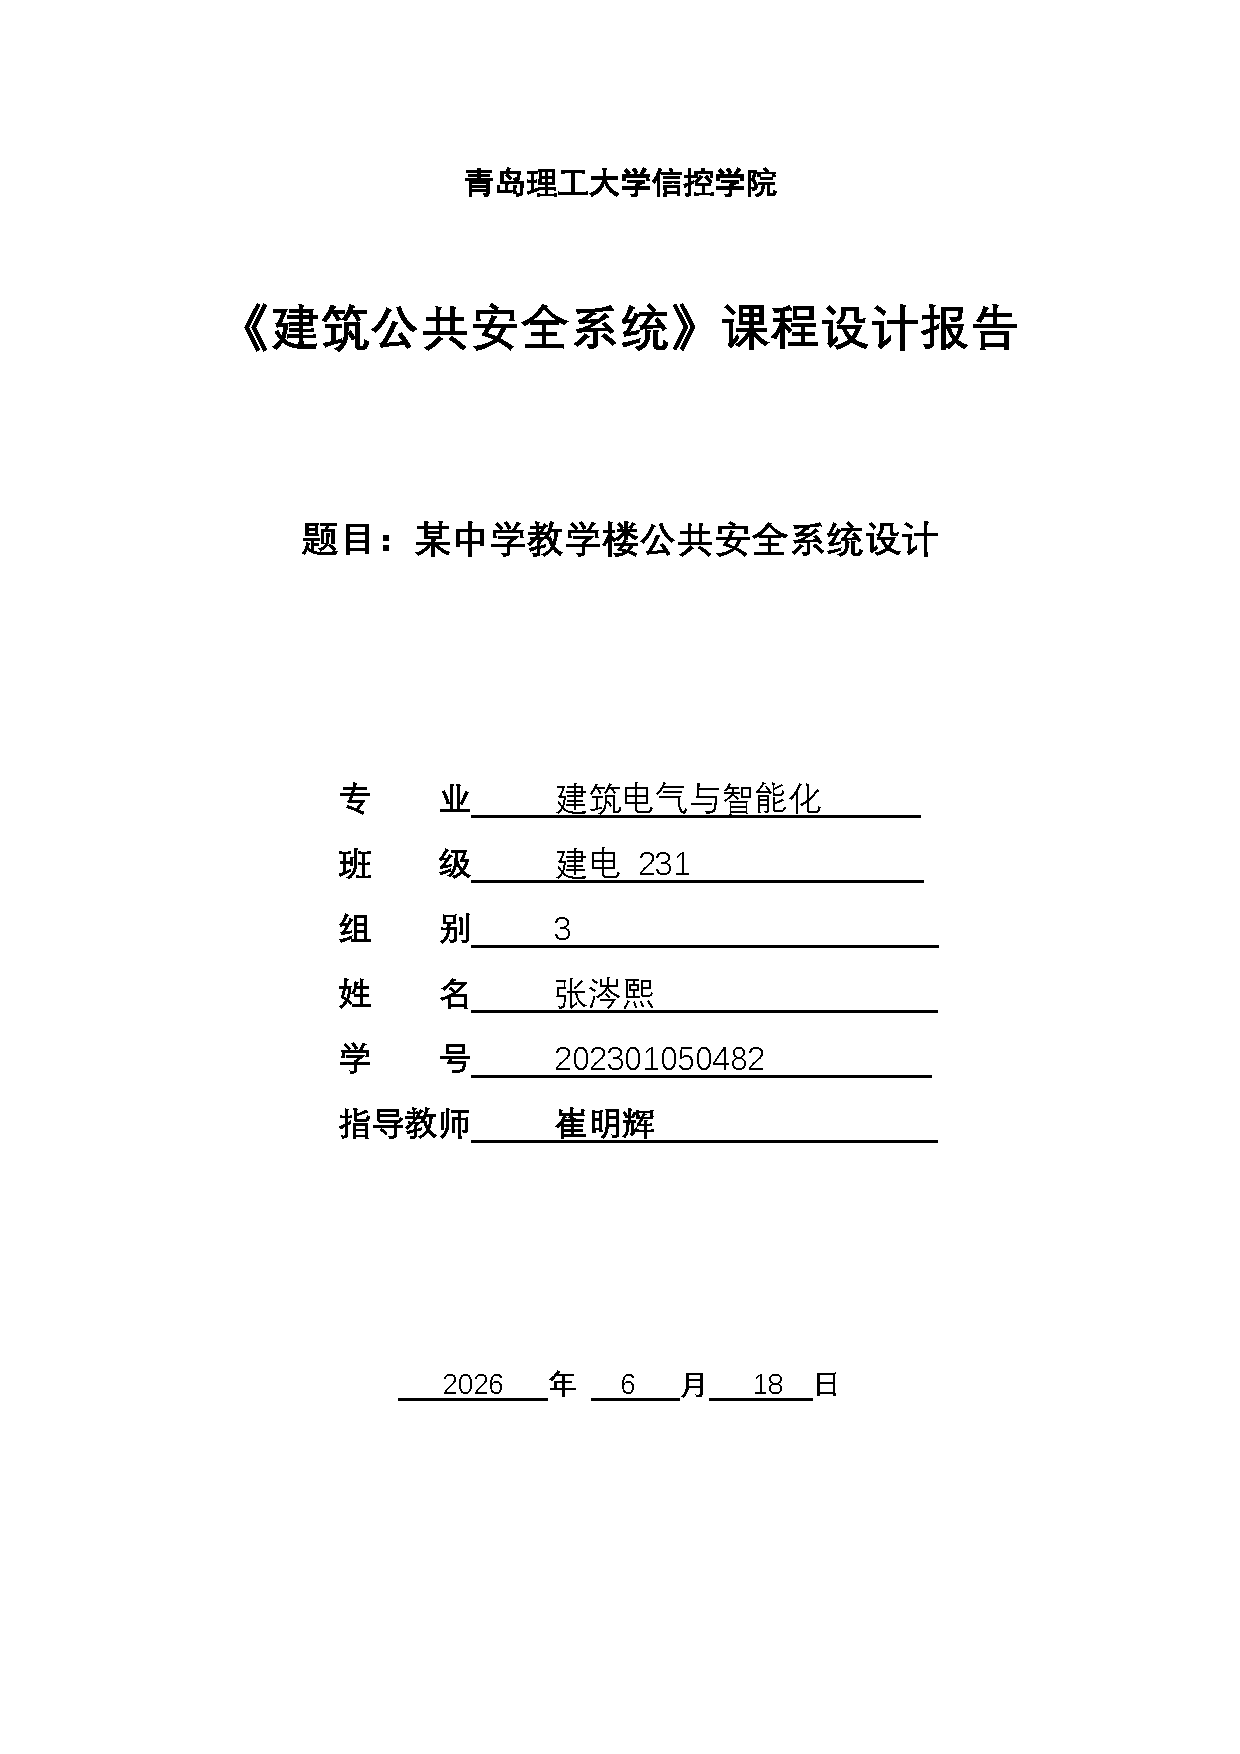
\includepdf[pages=-,pagecommand={\thispagestyle{empty}}]{建筑公共安全系统课程设计前两页.pdf}

\setcounter{page}{1}
\chapter*{摘\quad 要}
\addcontentsline{toc}{chapter}{摘要}
本设计以某学校1号教学楼、2号教学楼及行政办公楼为对象，完成建筑群视频安防监控系统设计。系统采用基于智能化网络的数字视频监控架构，前端设置1080P网络高清红外摄像机，重点覆盖各建筑出入口、走廊、楼梯间及行政办公楼安防控制室周边区域。监控中心设于行政办公楼一层安防消防控制室，配置视频管理服务器、集中存储设备、监控客户端、解码器及电视墙，实现实时监视、录像存储、检索回放和重点画面显示。

本设计共配置摄像机129台，其中室外红外枪式摄像机20台，室内红外半球摄像机109台。系统采用PoE接入交换机供电和传输，楼层交换机经汇聚交换机上联至行政办公楼监控中心。按单路视频码率4 Mbit/s、25帧/s、24小时连续录像、保存90天计算，录像原始容量约501.6 TB，考虑RAID、文件系统及20\%余量后，配置可用容量不小于602 TB的集中存储系统。报告完成了需求分析、系统方案、前端布点、传输网络、监控中心、供电、防雷接地、设备选型、容量计算和附录图纸。

\noindent\textbf{关键词：}公共安全；视频监控；网络摄像机；PoE；集中存储；安防控制室

\clearpage
\tableofcontents
\clearpage

\chapter{概述}
\section{工程概况}
本工程为某学校建筑群视频安防监控系统课程设计，设计对象包括1号教学楼、2号教学楼及行政办公楼。建筑功能以教学、办公、会议和公共交通空间为主，人员密度较高，出入口、走廊和楼梯间是日常管理、安全防范和事件追溯的重点区域。

监控中心设置在行政办公楼一层安防消防控制室。各建筑弱电间设置楼层PoE接入交换机，前端网络摄像机通过六类非屏蔽双绞线接入楼层交换机，再经建筑汇聚交换机上传至监控中心。系统采用数字视频监控方式，满足实时监视、集中管理、录像存储、事件检索和电视墙显示要求。

\section{需求分析}
根据课程设计任务书，本系统应实现以下功能：
\begin{enumerate}
  \item 对教学楼和行政办公楼主要出入口进行实时监视，记录人员进出情况。
  \item 对走廊、楼梯间等公共交通区域进行连续监控，减少监控盲区。
  \item 前端摄像机视频信号不低于25帧/s，显示、录像和回放清晰度按不低于1080P设计。
  \item 所有摄像机24小时不间断录像，录像资料保存90天。
  \item 监控中心能够进行画面切换、重点画面显示、录像检索、回放和权限管理。
  \item 系统采用UPS不间断电源供电，保证断电情况下关键设备短时持续运行。
\end{enumerate}

\section{设计依据}
本设计主要依据如下资料和规范：
\begin{enumerate}
  \item 《建筑公共安全系统课程设计任务书》。
  \item 《安全防范工程》15ZD09。
  \item 《安全防范工程技术标准》GB 50348。
  \item 《视频安防监控系统工程设计规范》GB 50395。
  \item 《民用建筑电气设计标准》GB 51348。
  \item 《综合布线系统工程设计规范》GB 50311。
  \item 原建筑电气底图和建筑功能分区资料。
\end{enumerate}

\section{设计内容}
本课程设计包括前端摄像系统、视频传输系统、视频控制系统、视频显示与记录系统四部分。具体内容包括摄像机布点、摄像机类型选择、PoE供电与传输网络设计、监控中心设备配置、存储容量计算、UPS容量估算、管线敷设方式及主要设备材料统计。

\chapter{系统设计}
\section{系统总体方案}
系统采用全数字网络视频监控架构，由前端网络摄像机、PoE接入交换机、建筑汇聚交换机、核心交换设备、视频管理服务器、集中存储设备、监控客户端、视频解码器和电视墙组成。摄像机通过Cat6 UTP线缆接入楼层PoE交换机，视频流经建筑汇聚交换机上传至行政办公楼安防控制室，由视频管理平台统一管理和存储。

\begin{figure}[H]
\centering
\resizebox{\textwidth}{!}{%
\begin{tikzpicture}[
  node distance=1.1cm and 1.35cm,
  box/.style={draw,rounded corners,align=center,minimum width=3.1cm,minimum height=0.9cm,fill=blue!6},
  core/.style={draw,rounded corners,align=center,minimum width=3.4cm,minimum height=1.0cm,fill=green!10},
  arr/.style={-{Stealth[length=2.5mm]},thick}
]
\node[box] (cam1) {1号教学楼\\52台摄像机};
\node[box,below=of cam1] (cam2) {2号教学楼\\46台摄像机};
\node[box,below=of cam2] (cam3) {行政办公楼\\31台摄像机};
\node[core,right=2.0cm of cam2] (agg) {建筑汇聚交换机\\10G光纤上联};
\node[core,right=2.0cm of agg] (core) {监控中心核心交换机\\视频专用VLAN};
\node[box,above=of core] (server) {视频管理服务器\\监控客户端};
\node[box,right=of core] (storage) {集中存储阵列\\90天录像};
\node[box,below=of core] (wall) {解码器\\电视墙显示};
\draw[arr] (cam1.east) -- node[above]{PoE/千兆接入} (agg.west);
\draw[arr] (cam2.east) -- (agg.west);
\draw[arr] (cam3.east) -- (agg.west);
\draw[arr] (agg.east) -- node[above]{10G OS2} (core.west);
\draw[arr] (core.north) -- (server.south);
\draw[arr] (core.east) -- (storage.west);
\draw[arr] (core.south) -- (wall.north);
\end{tikzpicture}
}
\caption{视频安防监控系统总体架构}
\end{figure}

\section{前端系统设计}
\subsection{摄像机布点原则}
摄像机布点遵循重点防护、连续覆盖、避免过度监控和便于维护的原则。出入口采用室外红外枪式摄像机，重点保证人脸方向、出入口宽度和夜间补光；走廊、楼梯间采用室内红外半球摄像机，兼顾视场角、安装美观和防拆需求。摄像机安装高度一般取2.6--3.5 m，室外出入口摄像机根据门厅和雨棚条件确定支架安装位置。

为保护师生隐私，摄像机不布置在卫生间、更衣空间、教师办公室内部和普通教室内部，仅覆盖公共安全管理需要的公共区域。

\subsection{摄像机数量统计}
\begin{longtable}{llrrrr}
\caption{摄像机布点统计}\label{tab:camera}\\
\toprule
建筑&楼层&室外枪机&室内半球&小计&主要覆盖区域\\
\midrule
\endfirsthead
\toprule
建筑&楼层&室外枪机&室内半球&小计&主要覆盖区域\\
\midrule
\endhead
1号教学楼&1F&6&8&14&主要出入口、门厅、走廊、楼梯间\\
&2F&0&10&10&走廊、楼梯间\\
&3F&0&10&10&走廊、楼梯间\\
&4F&0&10&10&走廊、楼梯间\\
&5F&0&8&8&走廊、楼梯间\\
\midrule
2号教学楼&1F&6&6&12&主要出入口、走廊、楼梯间\\
&2F&0&9&9&走廊、楼梯间\\
&3F&0&9&9&走廊、楼梯间\\
&4F&0&9&9&走廊、楼梯间\\
&5F&0&7&7&走廊、楼梯间\\
\midrule
行政办公楼&1F&8&2&10&主入口、安防控制室周边、走廊\\
&2F&0&7&7&走廊、楼梯间、会议区\\
&3F&0&7&7&走廊、楼梯间\\
&4F&0&7&7&走廊、楼梯间\\
\midrule
\multicolumn{2}{r}{合计}&20&109&129&\\
\bottomrule
\end{longtable}

\subsection{前端设备选型}
前端摄像机均采用1080P网络高清红外摄像机，支持H.265编码、ONVIF协议、PoE供电、三码流输出和本地时间叠加。室外出入口采用IP66防护等级枪式摄像机，室内公共区域采用红外半球摄像机。

\begin{table}[H]
\centering
\caption{前端摄像机选型}
\begin{tabularx}{\textwidth}{clXr}
\toprule
序号&设备&主要技术参数&数量\\
\midrule
1&室外红外枪式网络摄像机&1080P，25 fps，H.265，PoE，IP66，红外距离不小于30 m&20\\
2&室内红外半球网络摄像机&1080P，25 fps，H.265，PoE，红外距离不小于20 m，支持宽动态&109\\
\bottomrule
\end{tabularx}
\end{table}

\section{视频传输系统设计}
视频传输系统采用星形网络结构。前端摄像机至楼层PoE交换机采用Cat6 UTP线缆，传输距离控制在90 m以内。楼层PoE交换机接入建筑汇聚交换机，建筑汇聚交换机通过OS2单模光纤上联至行政办公楼监控中心核心交换机。监控业务独立划分视频专用VLAN，管理平台、存储设备和解码设备位于监控中心核心网络侧。

\subsection{网络带宽计算}
单路摄像机按4 Mbit/s主码流计算，实时预览、录像和回放均以主码流为基础。建筑上联带宽计算式为：
\begin{equation}
  B=N\times b
\end{equation}
式中，$B$为视频主码流带宽，$N$为摄像机数量，$b$为单路码率，取4 Mbit/s。

\begin{table}[H]
\centering
\caption{视频带宽计算}
\begin{tabular}{lrrr}
\toprule
建筑&摄像机数量&单路码率/Mbit/s&主码流带宽/Mbit/s\\
\midrule
1号教学楼&52&4&208\\
2号教学楼&46&4&184\\
行政办公楼&31&4&124\\
\midrule
合计&129&4&516\\
\bottomrule
\end{tabular}
\end{table}

系统总主码流带宽约516 Mbit/s。考虑平台访问、录像回放、码流波动和后期扩展，楼层接入采用千兆PoE端口，建筑汇聚至监控中心采用10G光纤链路，监控中心核心交换机采用万兆上联和千兆接入混合配置。

\subsection{交换设备配置}
各楼层按照摄像机数量设置24口PoE接入交换机，交换机预留不少于20\%端口余量。1号教学楼配置5台楼层PoE交换机，2号教学楼配置5台楼层PoE交换机，行政办公楼配置4台楼层PoE交换机，共14台。各建筑设置1台汇聚交换机，监控中心设置2台核心交换机，核心设备采用双机冗余。

\section{视频控制系统设计}
视频控制系统由视频管理服务器、管理平台软件、监控客户端、用户权限管理模块和时间同步模块组成。系统支持摄像机接入管理、实时预览、录像计划、录像检索、事件查询、设备状态监测、用户权限分级和日志记录。

视频管理平台设置于行政办公楼一层安防消防控制室。平台对所有摄像机统一编号，编号规则为“建筑-楼层-区域-序号”，例如“1J-01-N-01”表示1号教学楼一层北侧区域第1台摄像机。监控中心值班人员可按建筑、楼层、区域快速调用画面。

\section{视频显示和记录系统设计}
\subsection{显示系统}
监控中心设置监控客户端和电视墙。电视墙采用4块55英寸液晶拼接屏，配置视频解码器。系统可同时显示重点区域画面，并支持轮巡显示、报警联动显示和手动切换。显示画面应叠加时间、日期和监控地点，保证图像信息具有原始完整性。

\subsection{录像存储容量计算}
录像存储按所有摄像机24小时连续录像、保存90天计算。单路码率取4 Mbit/s，摄像机总数129台，原始存储容量计算式为：
\begin{equation}
  S=\frac{N\times b\times 3600\times 24\times D}{8\times 1000\times 1000}
\end{equation}
式中，$S$为原始容量，单位TB；$N$为摄像机数量；$b$为单路码率，单位Mbit/s；$D$为保存天数，取90天。

\begin{align*}
S &= \frac{129\times4\times3600\times24\times90}{8\times1000\times1000}\\
  &= 501.552\unit{TB}
\end{align*}

考虑RAID校验、文件系统开销、码流波动和20\%余量，存储配置容量为：
\begin{equation}
  S_c=501.552\times1.20=601.862\unit{TB}
\end{equation}
因此集中存储系统可用容量不应小于602 TB。工程配置可采用双控制器IPSAN/NVR集中存储，配置60块12 TB企业级硬盘并采用RAID6或同等冗余方式，满足90天录像保存和故障冗余要求。

\section{系统供电、防雷与接地}
摄像机通过PoE交换机集中供电，PoE接入交换机、汇聚交换机、核心交换机、服务器、存储和电视墙设备由UPS供电。UPS按监控中心核心设备功率和30 min后备时间配置，建议选用在线式UPS，容量不小于10 kVA。各弱电间PoE交换机接入楼层弱电UPS或应急电源回路。

室外摄像机及进入建筑物的线缆应设置浪涌保护措施。系统设备金属外壳、机柜、桥架和防雷保护器应可靠接地，接地电阻应满足建筑电气和弱电系统接地要求。

\section{管线敷设}
走廊区域视频线缆采用弱电桥架敷设，可与其他弱电线路共槽但应分区绑扎。由桥架引至摄像机处穿JDG20钢管暗敷或吊顶内敷设。室外摄像机引线应采用防水接线盒和金属管保护，穿墙处封堵防水。摄像机至交换机永久链路长度控制在90 m以内。

水平线缆按每台摄像机1根Cat6 UTP估算，平均长度按不同建筑取值并考虑10\%余量：
\begin{table}[H]
\centering
\caption{视频监控水平线缆估算}
\begin{tabular}{lrrr}
\toprule
建筑&摄像机数量&平均长度/m&估算线缆/m\\
\midrule
1号教学楼&52&45&2574\\
2号教学楼&46&40&2024\\
行政办公楼&31&35&1194\\
\midrule
合计&129&&5792\\
\bottomrule
\end{tabular}
\end{table}

Cat6线缆按305 m/箱配置，$5792/305=18.99$，向上取整并考虑施工损耗，配置20箱。

\chapter{设备选型与材料统计}
\section{主要设备配置}
\begin{longtable}{cllrr}
\caption{主要设备材料表}\\
\toprule
序号&设备名称&主要规格&单位&数量\\
\midrule
\endfirsthead
\toprule
序号&设备名称&主要规格&单位&数量\\
\midrule
\endhead
1&室外红外枪式网络摄像机&1080P，H.265，PoE，IP66&台&20\\
2&室内红外半球网络摄像机&1080P，H.265，PoE，宽动态&台&109\\
3&24口PoE接入交换机&千兆电口，PoE+供电，千兆/万兆上联&台&14\\
4&建筑汇聚交换机&千兆接入，万兆光上联&台&3\\
5&监控中心核心交换机&万兆光口，双机冗余&台&2\\
6&视频管理服务器&支持不少于200路摄像机管理&台&1\\
7&集中存储阵列&可用容量不小于602 TB，RAID冗余&套&1\\
8&监控客户端工作站&双屏显示，管理平台客户端&台&2\\
9&视频解码器&支持电视墙解码输出&台&1\\
10&55英寸拼接屏&监控中心电视墙&块&4\\
11&在线式UPS&不小于10 kVA，后备30 min&套&1\\
12&Cat6 UTP线缆&305 m/箱&箱&20\\
13&OS2单模光缆&12芯，建筑间主干&m&600\\
14&JDG20钢管&摄像机支线保护管&m&1200\\
15&弱电桥架&走廊主干敷设&m&按现场\\
\bottomrule
\end{longtable}

\section{系统特点}
本方案采用全数字网络视频监控系统，具有以下特点：
\begin{enumerate}
  \item 采用1080P网络高清摄像机，满足课程任务对清晰度和帧率的要求。
  \item 前端设备PoE供电，减少现场电源点，便于集中管理和维护。
  \item 监控业务独立VLAN传输，建筑间采用10G光纤上联，满足带宽和扩展需求。
  \item 集中存储按90天连续录像计算，容量配置有明确余量。
  \item 摄像机布点仅覆盖公共安全管理区域，兼顾安全防范和隐私保护。
\end{enumerate}

\chapter{课程设计总结}
本次课程设计以学校教学楼和行政办公楼为对象，完成了视频安防监控系统的方案设计。设计过程中首先分析建筑公共安全需求，确定出入口、走廊、楼梯间和安防控制室周边为重点监控区域；随后根据建筑数量、楼层和使用功能确定摄像机类型及数量；再完成传输网络、监控中心、录像存储、显示系统、供电和管线敷设设计。

通过本次设计，进一步掌握了视频安防监控系统的组成、网络化监控系统的设计方法、摄像机布点原则、码流与存储容量计算方法以及设备选型思路。设计中重点控制了两个问题：一是前端布点既要满足公共安全要求，又要避免对非公共区域过度监控；二是录像保存90天带来的存储容量较大，必须通过合理码率、集中存储和冗余配置保证系统可靠性。

本方案仍需在施工图深化阶段结合现场建筑尺寸、吊顶条件、门厅朝向和照明条件进一步校核摄像机视场角、安装高度、支架形式和管线路由。总体上，本设计满足课程任务书对系统架构、前端摄像、视频传输、视频控制、视频显示和录像保存的要求。

\chapter*{参考文献}
\addcontentsline{toc}{chapter}{参考文献}
\begin{enumerate}
  \item 《建筑公共安全系统课程设计任务书》.
  \item 《安全防范工程》15ZD09.
  \item GB 50348，安全防范工程技术标准.
  \item GB 50395，视频安防监控系统工程设计规范.
  \item GB 50311，综合布线系统工程设计规范.
  \item GB 51348，民用建筑电气设计标准.
\end{enumerate}

\appendix
\chapter{附录：系统图和平面布点图}
\includepdf[pages=-,pagecommand={}]{公共安全_附录_CAD图纸.pdf}

\end{document}
